\section{Organizzazione fisica della base di dati}

Un requisito fondamentale di un database è l'efficienza, cioè la capacità di rispondere alle 
richieste dell'utente il più rapidamente possibile: questo obiettivo può essere raggiunto grazie
ad una particolare organizzazione fisica dei dati. In questo capitolo verrà mostrato come il database
è organizzato a livello fisico, ovvero come questo viene salvato sull'unità di memoria 
di massa (disco rigido); nel prossimo paragrafo sarà quindi necessario illustrare brevemente come il
sistema operativo gestisce la lettura e scrittura di tale dispositivo.

\subsection{La memoria secondaria}
Il computer necessita di una \emph{memoria secondaria} dove poter salvare in modo permanente
i dati presenti nella RAM. Questa memoria secondaria è tipicamente un disco rigido, la cui struttura
meccanica è illustrata nella seguente figura.
\begin{center}
 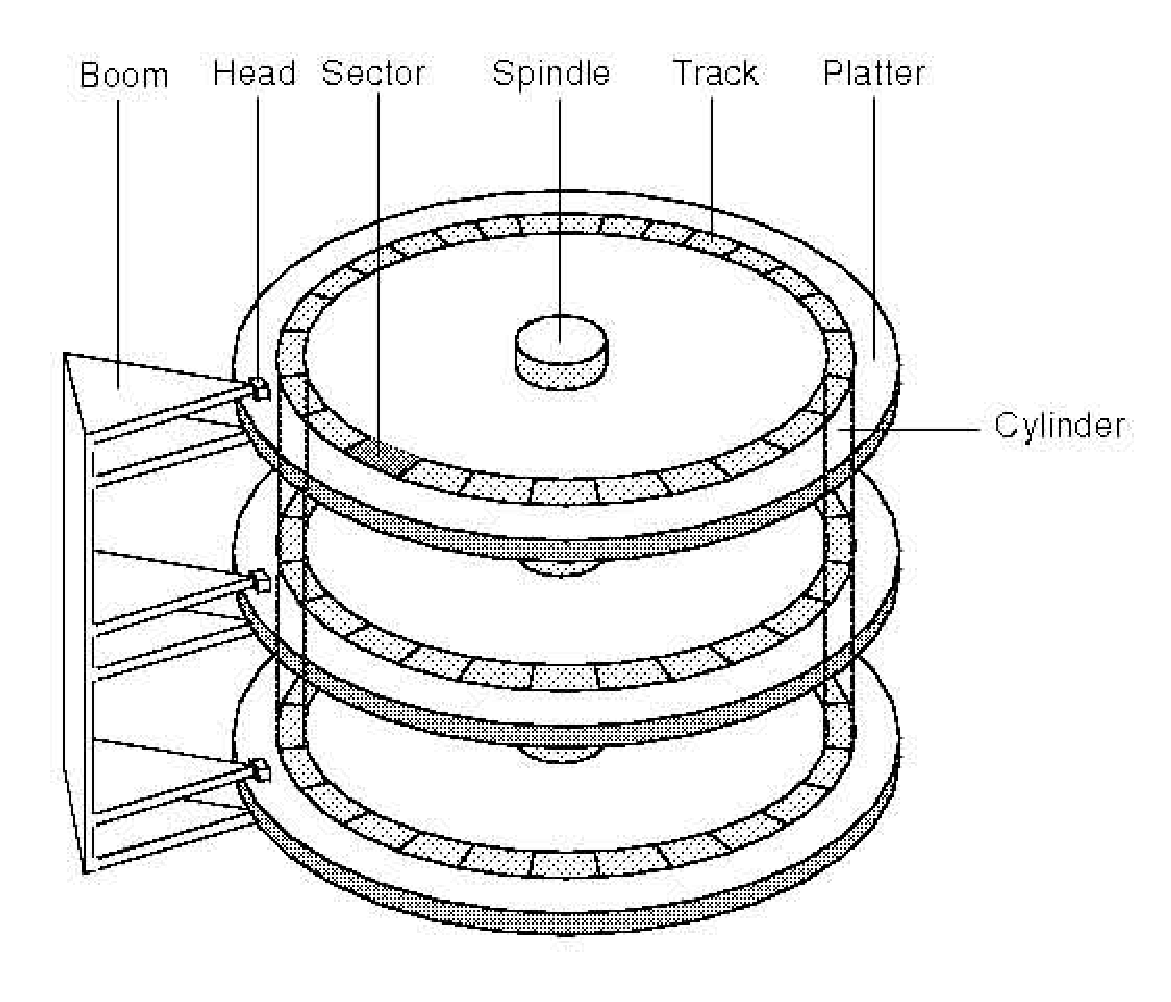
\includegraphics[width=300px]{immagini-eps/img_5_1.eps}
\end{center}
L'unità di memoria è composta da più \textbf{piatti}, di solito tre, ognuno dei quali è suddiviso
in \textbf{tracce}: esse sono come cerchi concentrici che partizionano tutta la superficie del
piatto. Al momento della \emph{formattazione}, durante la quale viede data una struttura logica per 
poter memorizzare i dati, impostando la struttura del filesystem che vi verrà creato sopra, vengono
creati i \textbf{settori} (o \textbf{blocchi} o pagine) di dimensione fissa, che varia da $2^9$ a $2^{12}$
bytes.\\
Quando si parla di \emph{accesso} al disco s'intende il trasferimento di un blocco da memoria secondaria 
a memoria principale, quindi \textbf{lettura} di un blocco, o da memoria principale a memoria secondaria, 
ossia \textbf{scrittura} di un blocco. Il tempo necessario per un accesso è dato dalla somma di:
\begin{itemize}
 \item \emph{tempo di posizionamento} della testina sulla traccia in cui si trova il blocco;
 \item \emph{ritardo della rotazione}, necessaria per posizionare la testina all'inizio del blocco;
 \item \emph{tempo di trasferimento} dei dati contenuti nel blocco.
\end{itemize}
Il tempo richiesto per un accesso a memoria secondaria è dell'ordine dei millisecondi, quindi 
notevolmente superiore a quello di elaborazione dei dati in memoria principale. Per questo motivo il 
\textbf{costo} di un'operazione sulla base di dati è definito in termini di \emph{numero di accessi}.

\subsection{Memorizzare le relazioni}

\subsubsection{Record}
Ad ogni relazione corrisponde un file di record che sono tutti dello stesso tipo (numero e 
tipo dei campi): ad ogni attributo corrisponde un \emph{campo}, che è di tipo elementare (interi,
reali, stringhe di caratteri), ed ad ogni tupla corrisponde un record. In un record, oltre ai campi 
che corrispondono agli attributi, ci possono essere altri campi che contengono informazioni sul 
record stesso o puntatori ad altri record.\\
Un \textbf{puntatore} ad un record è essenzialmente un dato che permette di accedere rapidamente a quel
record. Pertanto un puntatore può essere l'indirizzo dell'inizio (primo byte) del record su disco.
Tale scelta però può non essere adeguata se si vuole avere una certa libertà di muovere il record; in
questo caso è preferibile assumere come puntatore una coppia $(b, k)$ in cui $b$ è l'indirizzo del blocco
che contiene il record e $k$ è il valore di uno o più campi che servono come chiave nel file a cui il
record appartiene. In tal modo è possibile spostare il record all'interno del blocco. All'inizio di un 
record alcuni byte possono essere utilizzati per:
\begin{itemize}
 \item specificare il tipo del record, necessario quando in uno stesso blocco sono memorizzati 
 record di tipo diverso;
 \item specificare la lunghezza del record, se esso ha campi a lunghezza variabile;
 \item contenere un bit di ``cancellazione'', utile nel caso che il record sia puntato. In tal caso 
 lo spazio occupato dal record cancellato non può essere riutilizzato
 \item contenere un bit di ``usato/non usato'' per specificare se in quello spazio c'è un record oppure
 è vuoto (contiene valori casuali).
\end{itemize}

Per poter accedere ad un campo di un record contenente un dato è necessario sapere qual è il primo
byte del campo nel record. Se tutti i campi del record hanno lunghezza fissa, basta ordinarli; infatti,
una volta ordinati, l'inizio di ciascun campo sarà sempre ad un numero fisso di byte dall'inizio del
record: il numero di byte del record che precedono il campo è detto \textbf{offset} del campo. Se il record
contiene campi a lunghezza variabile allora l'offset di un campo può variare da un record all'altro.
In tal caso si possono usare due strategie:
\begin{itemize}
 \item all'inizio di ogni campo c'è un contatore che specifica la lunghezza del campo in numero di
byte
\item all'inizio del record ci sono gli offset di ciascun campo a lunghezza variabile (tutti i campi 
a lunghezza fissa precedono quelli a lunghezza variabile).
\end{itemize}

Nel primo caso per individuare la posizione di un campo bisogna esaminare i campi precedenti per
vedere quanto sono lunghi; quindi la prima strategia è meno efficiente della seconda. 

\subsubsection{Blocchi}
I record sono memorizzati nei blocchi. Analogamente a quanto accade per un record, anche in un blocco 
può essere riservato spazio per memorizzare informazioni sul blocco stesso (record cancellati, record 
non usati, puntatori a record se il blocco contiene record a lunghezza variabile), dello spazio 
``sprecato'' (per far in modo che gli offset di campi interi siano multipli di 4) o per collegarlo ad altri 
blocchi in una lista. Se un blocco contiene solo record di lunghezza fissa allora il blocco può essere 
suddiviso in aree (sottoblocchi) di lunghezza fissa ciascuna delle quali può contenere un record. Quando 
bisogna inserire un record nel blocco si cerca un area non usata; se il bit ``usato/non usato'' è in ciascun record
ciò può richiedere la scansione di tutto il blocco; per evitare ciò si possono raccogliere tutti i bit
``usato/non usato'' in uno o più byte all'inizio del blocco. 
In un blocco ci possono essere informazioni sul blocco stesso o puntatori ad altri blocchi.\\

Se un blocco contiene record di lunghezza variabile per accedere ai record si possono usare due
strategie:
\begin{itemize}
 \item si suppone che il primo record abbia inizio dal primo byte del blocco; si pone in ogni record un
campo che ne specifica la lunghezza in termini di numero di byte. Per calcolare il byte di inizio
di un record si somma all'offset del record precedente la sua lunghezza (ed eventualmente si
prende il successivo multiplo di 4);
 \item si pone all'inizio del blocco una \textbf{directory} contenente i puntatori ai record nel blocco 
 (in questo caso un puntatore è l'offset del record nel blocco). Poiché il numero di record che possono
entrare in un blocco è in questo caso variabile, la directory può essere realizzata in uno dei modi
seguenti:
\begin{itemize}
 \item la directory è preceduta da un campo che specifica quanti sono i puntatori nella directory
 \item la directory ha dimensione fissa (può contenere un numero fisso di puntatori) e contiene il
valore 0 (che non può essere un offset) negli spazi che non contengono puntatori (se il
numero di records nel blocco è inferiore al numero di puntatori che possono essere
memorizzati nella directory
\item la directory è una lista di puntatori (la fine della lista è specificata da uno 0).
\end{itemize}
\end{itemize}
L'uso di una directory all'inizio del blocco permette di spostare i record ``puntati''; infatti, basta 
far in modo che il puntatore invece di puntare al record punti al campo della directory che contiene
l'offset. Inoltre permette di spostare i bit di cancellazione dai record alla directory e quindi di
riutilizzare lo spazio occupato da un record a lunghezza variabile quando questo viene cancellato.

\subsection{File}
In questo paragrafo esamineremo diversi tipi di organizzazione fisica di file che consentono la
ricerca di record in base al valore di uno o più campi \emph{chiave}. Il termine ``chiave'' non va inteso nel
senso in cui viene usato nella teoria relazionale, in quanto un valore della chiave non necessariamente 
identifica univocamente un record nel file.
Le operazioni elementari su questi tipi di file sono dunque:
\begin{itemize}
 \item la ricerca di uno o più record con un dato valore per chiave;
 \item l'inserimento di un record con un dato valore per chiave;
 \item la cancellazione di uno o più record con un dato valore per chiave;
 \item la modifica di uno o più record con un dato valore per chiave. 
\end{itemize}

\subsubsection{Heap}
In questo tipo di organizzazione i record sono memorizzati nei blocchi senza alcun ordine: un
record viene sempre inserito come ultimo record del file. L'accesso al file avviene attraverso una
directory che contiene i puntatori ai blocchi; se le dimensioni lo consentono, tale directory può
essere mantenuta in memoria principale durante l'utilizzo del file; altrimenti saranno necessari
ulteriori accessi per portare in memoria principale i necessari blocchi della directory.
Denotiamo con $b$ il numero di blocchi del file ed esprimiamo in termini di $b$ il costo delle varie
operazioni, nella ipotesi che la directory si trovi in memoria principale.
Se la chiave di \textbi{ricerca} non identifica univocamente un record nel file, poiché non esiste alcun
particolare ordinamento dei record, per effettuare una ricerca occorre scandire tutto il file
sequenzialmente e, quindi, il costo di una ricerca è dato da $b$. L'\textbi{inserimento} di un record richiede la
lettura dell'ultimo blocco del file; se in tale blocco c'è spazio sufficiente per memorizzare il nuovo
record, il record viene inserito, altrimenti viene chiesto un nuovo blocco al file system; dopo
l'inserimento del record nel blocco, il blocco deve essere scritto su memoria secondaria. Quindi due
accessi (uno per lettura e uno per scrittura) sono sufficienti per l'inserimento di un record. La
\textbi{cancellazione} di tutti i record con un dato valore per la chiave richiede $b$ accessi in lettura 
per la ricerca di tutti i record che hanno quel valore per la chiave e $c$ accessi in scrittura, dove $c$ è il
numero di blocchi contenenti record con quel valore per la chiave; ulteriori accessi possono essere
necessari se si vuole recuperare lo spazio occupato dai record cancellati trasferendovi record che si
trovano nell'ultimo blocco. La \textbi{modifica} di tutti i record con un dato valore per la chiave richiede $b$
accessi in lettura per la ricerca di tutti i record che hanno quel valore per la chiave e $c$ accessi in
scrittura, dove $c$ è il numero di blocchi contenenti record con quel valore per la chiave.\\\\
Se la chiave di ricerca identifica univocamente un record nel file, la ricerca di un record con un dato
valore per la chiave richiede in media $[b/2]$ accessi. Per ottenere il costo medio occorre sommare i costi 
per accedere ai singoli record e quindi dividere tale somma per il numero dei record. Infatti, per la 
ricerca di un record che si trova nell'$i$-esimo blocco sono necessari $i$ accessi (in lettura); 
pertanto se denotiamo con $n$ il numero di record nel file e con $B$ il numero di record che possono 
essere memorizzati in un blocco ($[n/B]=b$), il numero medio di accessi necessari per la ricerca di un 
record è data da
\begin{center}
$\dfrac{B(1+2+\ldots +b)}{n} = \dfrac{Bb(b+1)}{2n} \simeq [b/2]$ 
\end{center}
(si osservi che $b/2\leq[b/2] \leq (b+1)/2$).\\
L'inserimento di un record richiede la lettura dell'ultimo blocco del file; se in tale blocco c'è spazio
sufficiente per memorizzare il nuovo record, il record viene inserito, altrimenti viene chiesto un
nuovo blocco al file system; dopo l'inserimento del record nel blocco, il blocco deve essere scritto
su memoria secondaria. Quindi 2 accessi (uno per lettura e uno per scrittura) sono sufficienti per
l'inserimento di un record. La cancellazione di un record con un dato valore per la chiave richiede
$[b/2]$ accessi in lettura per la ricerca del record che ha quel valore per la chiave e 1 accesso in
scrittura. Se si vuole recuperare lo spazio occupato dal record cancellato e i record hanno lunghezza
fissa si può trasferire un record che si trova nell'ultimo blocco (restituendo al sistema il blocco se
non vi sono altri record, in modo di ridurre i costi delle successive operazioni sul file) al posto di
quello cancellato. Se si vuole recuperare lo spazio occupato dal record cancellato e i record hanno
lunghezza variabile, si possono far slittare i record nel blocco (aggiornando i puntatori ai record
nell'intestazione del blocco) e, se in tal modo si è ottenuto uno spazio sufficiente per trasferirvi un
record che si trova nell'ultimo blocco, procedere come nel caso precedente. La modifica di un
record con un dato valore per la chiave richiede $[b/2]$ accessi in lettura per la ricerca del record che
ha quel valore per la chiave e 1 accesso in scrittura.\\

\subsubsection{File hash}
In questo tipo di organizzazione i record sono ripartiti in \textbf{bucket} (secchi) in base al valore della
chiave. Se $B$ è il numero dei bucket, questi vengono numerati da $1$ a $B$. Dato un valore $v$ per
chiave il numero del bucket in cui deve trovarsi un record con chiave $v$ è calcolato mediante una
funzione che prende il nome di \emph{funzione hash}.
Ciascun bucket è costituito da uno o più blocchi (come vedremo, affinchè la gestione del file sia
efficiente è opportuno che il numero dei blocchi in un bucket sia piccolo) ed è organizzato come un
heap. L'accesso ai bucket avviene attraverso la bucket directory che contiene $B$ elementi
(normalmente $B$ è sufficientemente piccolo da consentire di mantenere la bucket directory in
memoria principale durante l'utilizzo del file); l'$i$-esimo elemento contiene l'indirizzo (bucket
header) del primo blocco dell'$i$-esimo bucket. Tutti i blocchi di un bucket sono collegati tra loro
mediante puntatori in una lista.
Una funzione hash per essere ``buona'' deve ripartire uniformemente i record nei bucket, cioè al
variare del valore della chiave deve assumere con la ``stessa'' probabilità uno dei valori compresi tra
$0$ e $B-1$. Esiste un'ampia letteratura sulle funzioni hash. In genere, una funzione hash trasforma la
chiave in un intero, divide questo intero per $B$, e fornisce il resto della divisione come numero di
bucket in cui deve trovarsi il record con quel valore della chiave. Una strategia per definire una
funzione hash è, ad esempio, la seguente:
\begin{enumerate}
 \item trattare il valore v della chiave come una sequenza di bit
 \item suddividere tale sequenza in gruppi di bit di uguale lunghezza
 \item sommare tali gruppi trattandoli come interi
 \item dividere il risultato per il numero dei bucket (cioè per $B$)
 \item prendere il resto della divisione come numero del bucket in cui deve trovarsi un record con
chiave $v$.
\end{enumerate}

Una qualsiasi operazione (ricerca, inserimento, cancellazione, modifica) su un file hash richiede la
valutazione di $h(v)$ (dove $v$ è un valore per la chiave e $h$ è la funzione hash) per individuare il bucket
in cui deve trovarsi il record con chiave $v$; successivamente, l'operazione (ricerca, inserimento,
cancellazione, modifica) viene effettuata sul bucket che, come già detto, è organizzato come un
heap. Se la funzione hash distribuisce uniformemente i record nei bucket, ogni bucket è costituito
da un numero di blocchi che è $1/B$-esimo del numero di blocchi di cui è costituito l'intero file.
Pertanto il costo richiesto per un'operazione è approssimativamente $1/B$-esimo del costo che
sarebbe richiesto per fare la stessa operazione se il file fosse organizzato come un heap. Si osservi
che, poiché l'inserimento di un record viene effettuato sull'ultimo blocco del bucket, è opportuno
che la bucket directory contenga anche, per ogni bucket, un puntatore all'ultimo record del bucket.
Da quanto detto appare evidente che quanti più sono i bucket tanto più basso è il costo di ogni
operazione. D'altra parte limitazioni al numero dei bucket derivano dalle seguenti considerazioni:
\begin{enumerate}
 \item ogni bucket deve avere almeno un blocco
\item se le dimensioni della bucket directory sono tali che non può essere mantenuta in memoria
principale durante l'utilizzo del file, ulteriori accessi sono necessari per leggere i blocchi della
bucket directory.
\end{enumerate}

\subsubsection{File con indice (indice sparso)}
Nella presentazione di questo tipo di organizzazione, spesso chiamato \emph{ISAM} (Indexed Sequential
Access Method), assumeremo che il valore della chiave identifica univocamente un record del file.
Inoltre, inizialmente, assumeremo che i record non siano puntati.\\\\
Inizialmente il file viene ordinato in base al valore (crescente) della chiave e viene memorizzato
lasciando in ogni blocco una certa percentuale (ad esempio il 20\%) di spazio non utilizzato per
l'inserimento di nuovi record; quindi viene creato un nuovo file, il \textbf{file indice} che
contiene un record per ogni blocco del file principale, e infine la directory del file indice che 
generalmente ha dimensioni tali da poter essere mantenuta in memoria principale durante l'utilizzo del file.\\
Un file indice è un file i cui record consistono di coppie del tipo $(v, b)$, in cui $v$ è un valore della
chiave e $b$ è l'indirizzo di un blocco del file principale: il valore della chiave di ogni record nel
blocco di indirizzo $b$ è maggiore o uguale a $v$ e il valore della chiave di ogni record che si trova in
un blocco che precede quello di indirizzo $b$ è minore di $v$.\\
Il file indice viene creato nel modo seguente. Per ogni blocco del file principale viene creata una
coppia costituita dal valore della chiave del primo record nel blocco e dall'indirizzo del blocco;
l'unica eccezione è rappresentata dal primo blocco per il quale viene preso, anziché il valore della
chiave del primo record, un valore (denotato con $-\infty$) che è più piccolo di qualsiasi valore che può
essere assunto dalla chiave.\\
L'accesso al file principale avviene attraverso il file indice nel modo seguente. Dato un valore $v$
della chiave, si cerca nel file indice un valore $v'$ della chiave che \emph{ricopre} $v$, cioè una coppia 
$(v', b')$ aventi le seguenti proprietà:
\begin{itemize}
 \item $v' \leq v$
 \item o $(v', b')$ è l'ultimo record del file indice oppure, se $(v'', b'')$ è il successivo record 
 nel file indice, $v<v''$.
\end{itemize}

Il blocco che ha per indirizzo $b'$ è allora il blocco in cui deve trovarsi il record con chiave $v$.
Pertanto la ricerca di un record con chiave $v$ richiede un accesso in più oltre quelli necessari per la
ricerca nel file indice di un valore della chiave che ricopre $v$.
La chiave del file principale è una chiave anche per il file indice; pertanto i record del file indice
possono a loro volta essere ordinati in base al valore della chiave. Il fatto che il file indice sia
ordinato in base al valore della chiave consente di usare metodi più efficienti della scansione
completa per ricercare sul file indice un valore della chiave che ricopra un dato valore $v$.
Il più semplice è costituito dalla \textbf{ricerca binaria}.\\ Siano $B_1, B_2, \ldots, B_m$ i blocchi del file indice; si
comincia con il considerare il blocco $B_{[m/2]}$ e si confronta il valore $w$ della chiave nel primo record
di tale blocco con $v$; se $v = w$ la ricerca ha termine; se $v < w$ si ripete il procedimento come se il file
indice fosse costituito dai blocchi $B_1, B_2, \ldots, B_{[m/2]-1}$; se invece $v > w$ e nel blocco esiste un valore
della chiave che ricopre $v$ la ricerca ha termine, altrimenti si ripete il procedimento come se il file
indice fosse costituito dai blocchi $B_{[m/2]}, \ldots, B_m$. Il procedimento viene iterato fino a quando
ci si riduce a considerare un unico blocco; a questo punto si scandisce il blocco per trovare un
valore della chiave che ricopre $v$. Poiché ad ogni passo il numero di blocchi su cui deve essere
effettuata la ricerca viene dimezzato, dopo al più $[log_2(m)]$ passi la ricerca è ristretta ad un unico
blocco.\\
Un altro metodo è costituito dalla \textbf{ricerca per interpolazione}. Questo tipo di ricerca è basato sulla
conoscenza della distribuzione dei valori della chiave. In altre parole per poter effettuare questa
ricerca si deve disporre di una funzione $f$ che dati tre valori $v_1, v_2, v_3$ della chiave fornisce un valore
che è la frazione dell'intervallo di valori della chiave compresi tra $v_2$ e $v_3$ in cui deve trovarsi $v_1$. 
In tal caso, se $B_1, B_2, \ldots, B_m$ sono i blocchi del file indice (o di una sua parte) e $v_2$ è il valore della
chiave nel primo record di $B_1$ e $v_3$ è il valore della chiave nell'ultimo record di $B_m$ allora $v_1$ deve
essere confrontato con il valore della chiave nel primo record di $B_i$, dove $i = mf(v_1, v_2, v_3)$;
analogamente a quanto accade nella ricerca binaria, se $v_1$ è minore di tale valore allora il
procedimento deve essere ripetuto sui blocchi $B_1, B_2, \ldots, B_{i-1}$, mentre se è maggiore il procedimento
deve essere ripetuto sui blocchi $B_i, B_{i+1}, \ldots, B_m$, finchè la ricerca si restringe ad un unico blocco. \`E
stato mostrato che la \textbi{ricerca} per interpolazione richiede circa $1+log_2(log_2(m))$ accessi.\\
Per \textbi{inserire} un nuovo record nel file principale occorre innanzitutto ricercare il blocco $B_i$ del file
principale in cui il record deve trovarsi in base al valore della chiave. Se in $B_i$ c'è spazio sufficiente,
il record viene inserito in modo da rispettare l'ordinamento (quindi spostando eventualmente
record con chiave maggiore). Altrimenti si possono seguire diverse strategie. Ad esempio si può
verificare se c'è spazio sufficiente nel blocco successivo $B_{i+1}$; in tal caso, o il nuovo record o un
record che era precedentemente in $B_i$ diventa il primo record di $B_{i+1}$ e, pertanto, il record del file
indice che contiene il puntatore a $B_{i+1}$ deve essere modificato. Se $B_{i+1}$ non esiste ($B_i$ è l'ultimo
blocco del file) oppure è pieno si può prendere in considerazione il blocco $B_{i-1}$ ed eventualmente
procedere in modo simile ripartendo i record di tra $B_{i-1}$ e $B_i$; anche in questo caso sarà necessario
apportare una modifica al file indice. Se anche $B_{i-1}$ è pieno oppure se $B_{i-1}$ non esiste ($B_i$ è il primo
blocco del file), è necessario richiedere al sistema un nuovo blocco che seguirà $B_i$ e ripartire i
record di $B_i$ tra $B_i$ e il nuovo blocco; quindi occorre inserire nel file indice il record relativo al
nuovo blocco. In ogni caso occorrerà modificare i bit di ``usato/non usato'' nelle intestazioni dei blocchi coinvolti.\\
Per \textbi{cancellare} un record dal file principale occorre innanzitutto ricercare il record, quindi
cancellarlo, spostare i record nel blocco in modo da recuperare lo spazio lasciato libero e modificare
i bit di ``usato/non usato'' nell'intestazione del blocco. Se il record cancellato è il primo record del
blocco occorre modificare nel file indice il record relativo al blocco. Se il record cancellato era
l'unico record del blocco, il blocco viene restituito al sistema e nel file indice occorre cancellare il
record relativo al blocco (anche in questo caso se il record cancellato è l'unico record del blocco, il
blocco viene restituito al sistema). In ogni caso occorrerà modificare i bit di ``usato/non usato'' nelle 
intestazioni dei blocchi coinvolti.\\
Per \textbi{modificare} un record del file principale occorre innanzitutto ricercare il record; quindi, se la
modifica non coinvolge campi della chiave, il record viene modificato e il blocco riscritto. Altrimenti la modifica 
equivale ad una cancellazione seguita da un inserimento.\\\\
Consideriamo ora il caso in cui il file principale contiene record puntati. In tal caso la fase di inizializzazione 
non differisce dal caso precedente salvo che è preferibile lasciare più spazio libero nei blocchi per successivi inserimenti. 
Infatti, poiché i record sono puntati, non possono essere spostati per mantenere l'ordinamento quando si inseriscono nuovi record;
pertanto, se non c‘è spazio sufficiente in un blocco $B$ per l'inserimento di un nuovo record, occorre
richiedere al sistema un nuovo blocco che viene collegato a $B$ tramite un puntatore; in tal modo
ogni record del file indice punta al primo blocco di un bucket e il file indice non viene mai
modificato (a meno che le dimensioni dei bucket non siano diventate tali da richiedere una
riorganizzazione dell'intero file). La ricerca di un record con chiave $v$ richiede la ricerca sul file
indice di un valore della chiave che ricopre $v$ e quindi la scansione del bucket corrispondente. La
cancellazione di un record richiede la ricerca del record e quindi la modifica dei bit di cancellazione
nell'intestazione del blocco. La modifica di un record richiede la ricerca del record; quindi, se la
modifica non coinvolge campi della chiave, il record viene modificato e il blocco riscritto.
Altrimenti la modifica equivale ad una cancellazione seguita da un inserimento. In quest'ultimo
caso non è sufficiente modificare il bit di cancellazione del record cancellato, ma è necessario
inserire in esso un puntatore al nuovo record inserito in modo che questo sia raggiungibile da
qualsiasi record che contenga un puntatore al record cancellato.
Poiché non è possibile mantenere il file principale ordinato, se si vuole avere la possibilità di
esaminare il file seguendo l'ordinamento della chiave occorre inserire in ogni record un puntatore al
record successivo nell'ordinamento.

\subsubsection{B-tree}
Questa organizzazione è una generalizzazione del file con indice. Infatti in un file con indice,
attraverso una ricerca sul file indice, viene individuato il blocco del file principale in cui deve
trovarsi il record con un dato valore per la chiave. In un B-tree si accede al file attraverso una
\emph{gerarchia} di indici. L'indice a livello più alto nella gerarchia è costituito da un unico blocco e quindi
può risiedere in memoria principale durante l'utilizzo del file. Durante la ricerca di un record con un
dato valore per la chiave si accede agli indici a partire da quello a livello più alto; a mano a mano
che si scende nella gerarchia di indici si restringe la porzione (insieme di blocchi) del file principale
in cui deve trovarsi il record desiderato, fino a che, nell'ultimo livello (il più basso nella gerarchia)
tale porzione è ristretta ad un unico blocco. I blocchi degli indici e del file principale devono essere
sempre pieni almeno per metà.\\
Ogni blocco di un file indice è costituito di record contenenti una coppia $(v, b)$ dove $v$ è il valore
della chiave del primo record della porzione del file principale che è accessibile attraverso il
puntatore $b$; $b$ può essere un puntatore ad un blocco del file indice a livello immediatamente più
basso oppure (nei record del file indice nel più basso livello della gerarchia) ad un blocco del file
principale.\\
Per \textbi{ricercare} il record del file principale con un dato valore $v$ per la chiave si procede nel modo
seguente. Si parte dall'indice a livello più alto (che è costituito da un unico blocco) e ad ogni passo
si esamina un unico blocco. Se il blocco esaminato è un blocco del file principale, tale blocco è
quello in cui deve trovarsi il record desiderato; se, invece, è un blocco di un file indice, si cerca su
tale blocco un valore della chiave che ricopre $v$ e si segue il puntatore associato (che sarà o un
puntatore ad un blocco dell'indice al livello immediatamente inferiore o un blocco del file
principale). Per valutare il costo di un'operazione di ricerca, assumiamo, per comodità, che il
numero di record del file principale che possono essere memorizzati in un blocco sia un numero
dispari $2e-1$, che il numero di record di un file indice che possono essere memorizzati in un blocco
sia un numero dispari $2d-1$ (cioè, poiché ogni blocco è pieno almeno per metà, ogni blocco del file
principale contiene almeno $e$ record e ogni blocco di un indice contiene almeno $d$ record). Con tali
assunzioni il file principale ha al più $n/e$ blocchi, dove $n$ è il numero di record del file principale.
Poiché ad ogni blocco del file principale corrisponde un record nel file indice al livello $1$ (il più
basso nella gerarchia) il numero di record del file indice a livello più basso sarà $n/e$ e, per l'ipotesi
fatta (ogni blocco è pieno almeno per metà), questi $n/e$ record saranno memorizzati in al più $n/(ed)$
blocchi. Ripetendo tale ragionamento, si ottiene che l'indice a livello $i$ ha $n/(ed^{i-1})$ record
memorizzati in al più $n/(ed^i)$ blocchi. Sia $k$ il livello più alto della gerarchia; l'indice a livello
$k$ avrà $n/(ed^{k- 1})$ record memorizzati in al più $n/(ed^k)$ blocchi; poiché tale indice è costituito 
da un unico blocco $n/(ed^k)\geq 1$. Poiché per ricercare un record del file principale si deve accedere 
ad un blocco per ogni livello di indice più al blocco del file principale che contiene il record 
desiderato, il numero di accessi necessari per un operazione di ricerca è $k +1 \leq log_d(n/e)+1$.\\
Il numero di accessi necessari per effettuare l'inserimento del record con valore $v$ della chiave è
dato dal numero di accessi necessari per ricercare il blocco in cui deve essere inserito il record con
chiave $v$ più uno per riscrivere il blocco, se nel blocco c'è spazio sufficiente per inserire il record.
Se, viceversa, nel blocco non c'è spazio sufficiente per inserire il nuovo record, l'operazione di
inserimento può richiedere un numero ulteriore di accessi a causa della necessità di mantenere i
blocchi pieni al meno per metà, come mostra il seguente esempio. Si osservi che, per salvare spazio,
il primo record in ogni blocco di un file indice è costituto da un puntatore anziché da una coppia
chiave-puntatore; tale puntatore permette di accedere alla parte del file principale contenente record
con valore della chiave minore del valore presente nel secondo record del blocco del file indice.
Supponiamo che in un certo istante la configurazione del B-tree sia la seguente:
\begin{figure}[h!]
  \centering
  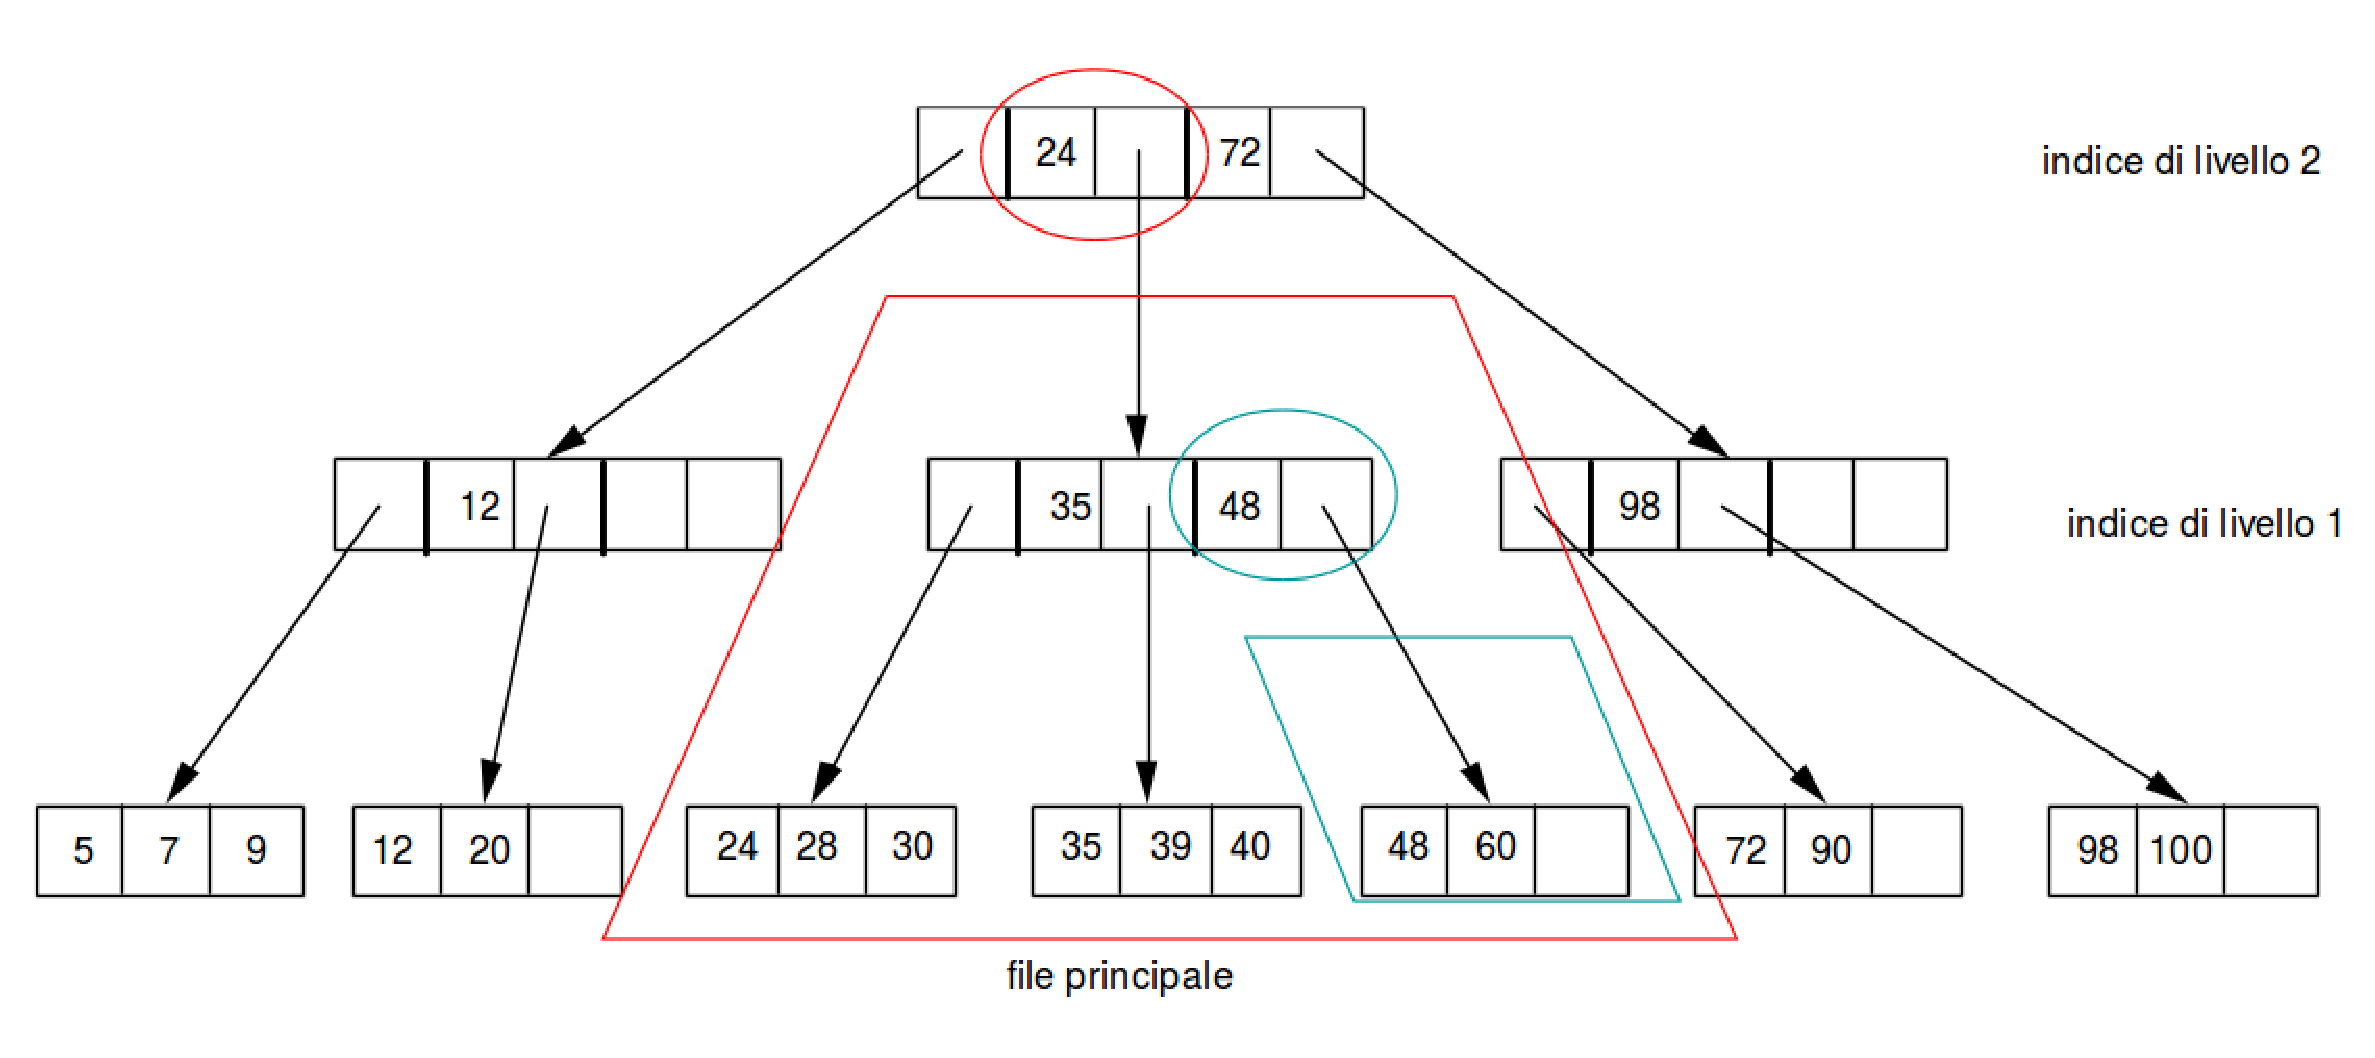
\includegraphics[width=430px]{immagini-eps/img_5_3_4(1).eps}
  Figura 1
\end{figure}

e che si voglia inserire il record con valore della chiave $25$. Poiché il blocco (il terzo da sinistra) del
file principale in cui dovrebbe essere inserito tale record è pieno occorre richiedere al sistema un
nuovo blocco e ripartire i record del terzo blocco e il nuovo record fra il terzo blocco e il nuovo
blocco in modo da soddisfare il vincolo che ogni blocco deve essere pieno almeno per metà. Inoltre,
poiché il blocco del file indice di primo livello in cui dovrebbe essere inserito il puntatore al nuovo
blocco del file principale è pieno, occorre procedere per il file indice di livello $1$ allo stesso modo in
cui si è proceduto per il file principale, richiedendo un nuovo blocco al sistema. Ma allora un
analogo discorso deve essere fatto per l'indice di livello $2$. Pertanto dopo l'inserimento del record
con chiave $25$ il B-tree si presenterà come segue:

\begin{figure}[h!]
  \centering
  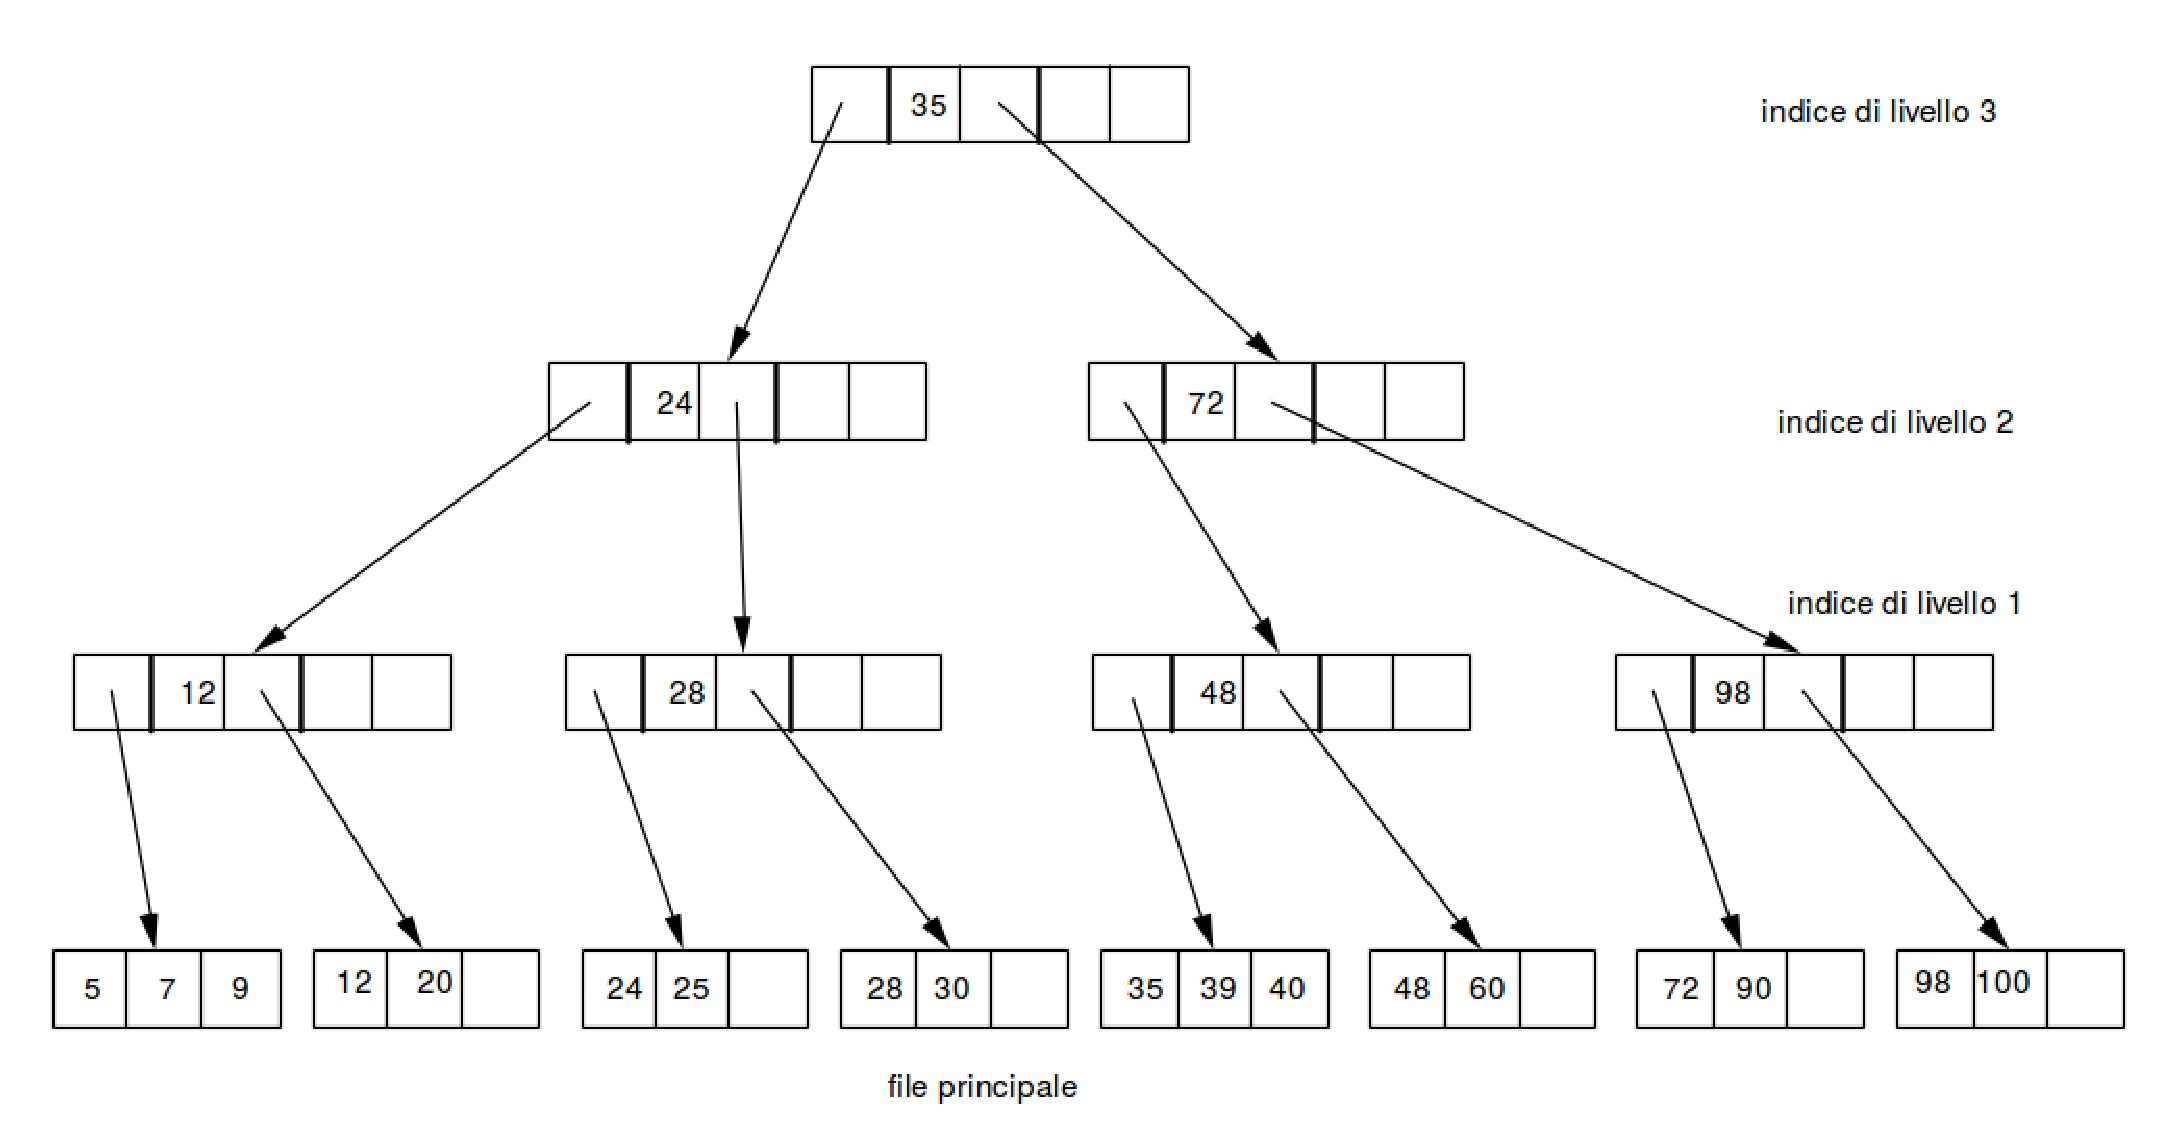
\includegraphics[width=430px]{immagini-eps/img_5_3_4(2).eps}
  Figura 2
\end{figure}

Come si vede il numero dei livelli degli indici è aumentato di $1$, il che comporta un aumento dei
costi delle successive operazioni sul file principale.
Il numero di accessi necessari per effettuare la cancellazione del record con valore $v$ della chiave è
dato dal numero di accessi necessari per ricercare il blocco in cui si trova il record con chiave v più
uno per riscrivere il blocco, se il blocco rimane pieno almeno per metà successivamente alla
cancellazione. Se, viceversa, il blocco non rimane pieno almeno per metà successivamente alla
cancellazione, l'operazione può richiedere un numero ulteriore di accessi come mostra il seguente
esempio.\\
Supponiamo che in un certo istante la configurazione del B-tree sia quella mostrata in \textsc{Figura 2} e che si
voglia cancellare il record con chiave $28$. Poiché, a seguito della cancellazione di tale record nel
blocco rimane un solo record (e quindi non è soddisfatto il vincolo che ogni record debba essere
pieno al meno per metà), e tale record può trovare posto nel blocco precedente (il terzo da sinistra),
il blocco può essere restituito al sistema. Inoltre, poiché nel secondo blocco dell'indice di livello 1
rimane un solo puntatore possiamo procedere per l'indice di livello $1$ analogamente a come si è
proceduto per il file principale. Ma allora un analogo discorso deve essere fatto per l'indice di
livello $2$. Pertanto dopo la cancellazione del record con chiave $28$ il B-tree si presenterà come segue:

\begin{figure}[h!]
  \centering
  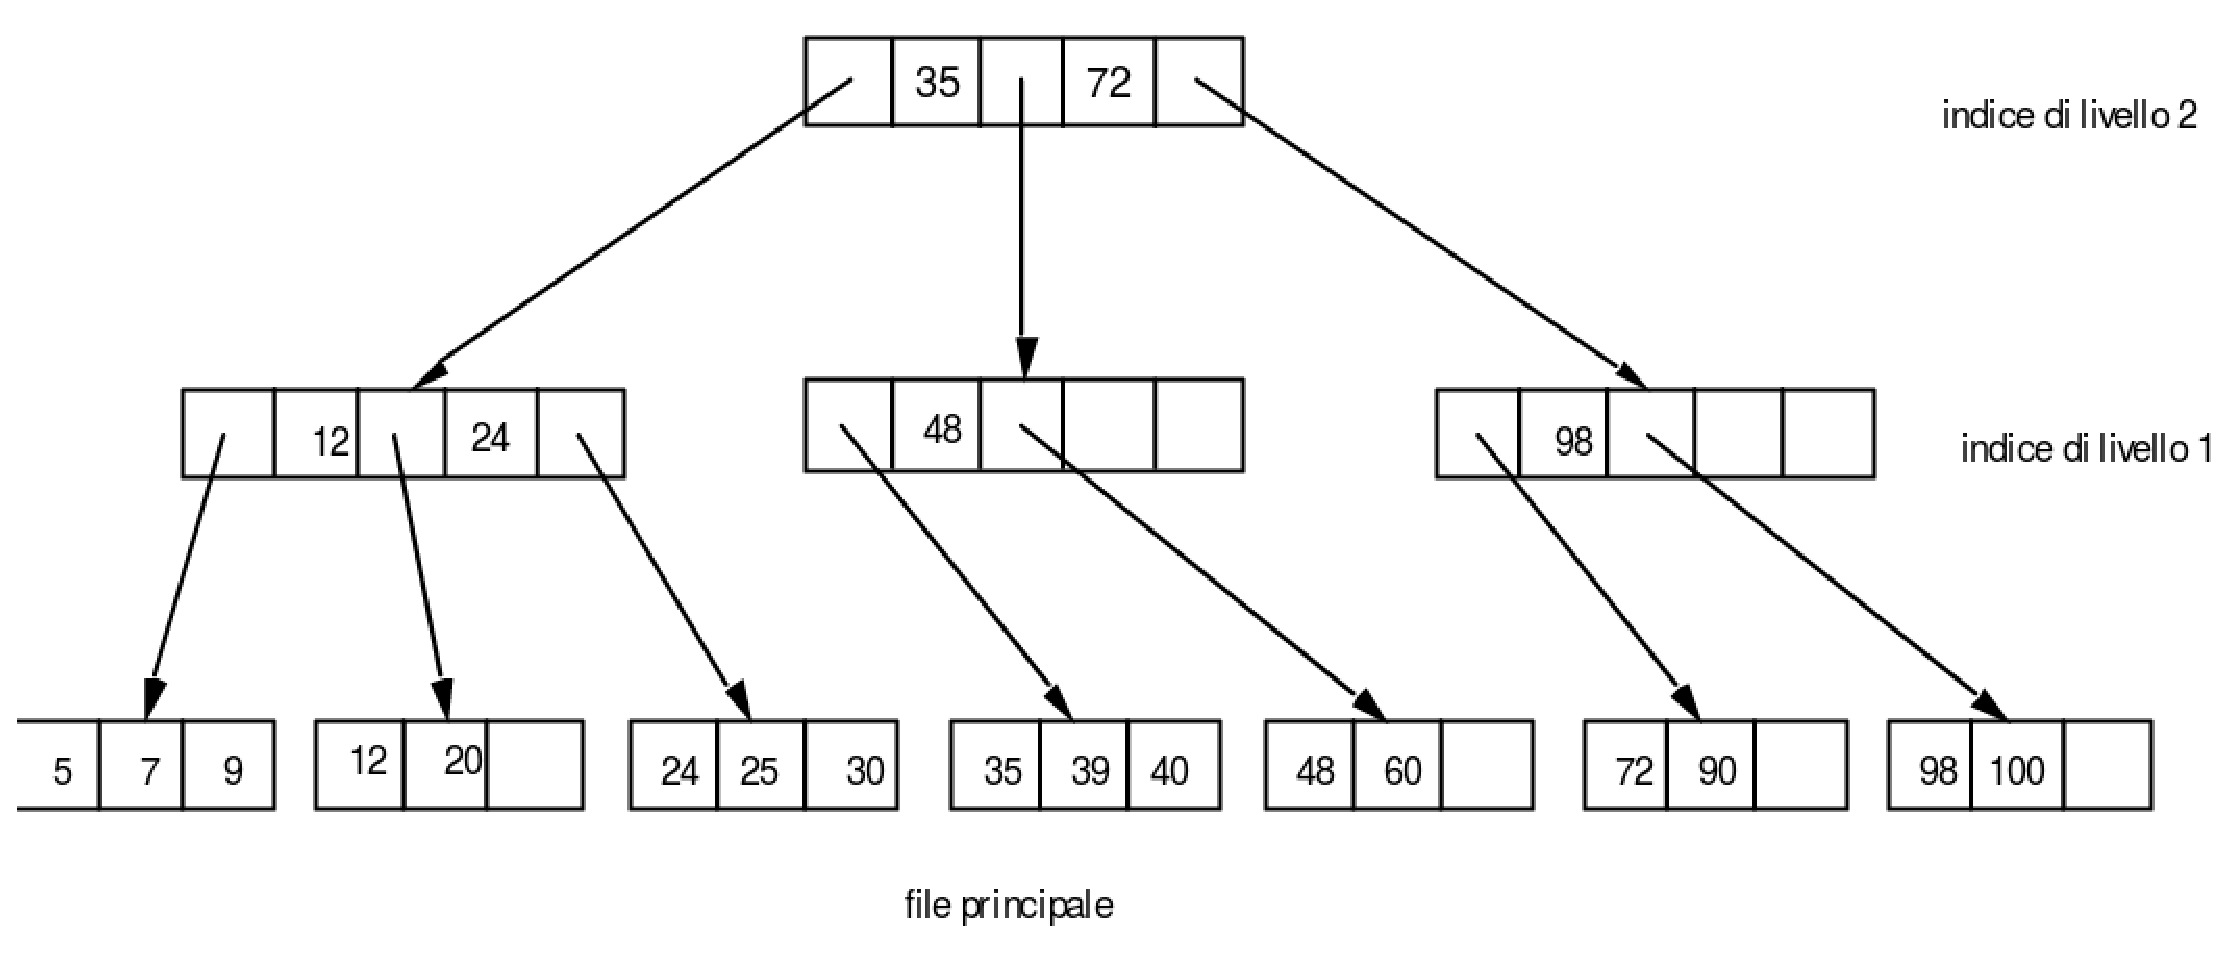
\includegraphics[width=400px]{immagini-eps/img_5_3_4(3).eps}
  Figura 3
\end{figure}

Come si vede il numero dei livelli degli indici è diminuito di $1$, il che comporta una diminuzione dei
costi delle successive operazioni sul file principale.
Il numero di accessi necessari per effettuare la modifica del record con valore $v$ della chiave è dato
dal numero di accessi necessari per ricercare il blocco in cui si trova il record con chiave $v$ più uno
per riscrivere il blocco, se la modifica non coinvolge campi della chiave, altrimenti è dato dalla
somma degli accessi necessari per la cancellazione del record con chiave $v$ e quelli necessari per
l'inserimento del record con il nuovo valore della chiave.

\subsubsection{File con indice denso}
Nelle organizzazioni viste nei paragrafi precedenti, escluso l'heap, la maggior parte dei blocchi del
file principale non sono riempiti completamente; ciò comporta spreco di memoria e aumento dei
tempi di ricerca. D'altra parte, in un heap i blocchi sono completamente pieni, ma non si ha un
metodo efficiente per la ricerca di un record con un dato valore per la chiave.
Un tipo di organizzazione che cerca di cogliere gli aspetti positivi dell'uno e degli altri tipi di
organizzazione è il \textbf{file con indice denso}. Mentre nel caso di un file con indice sparso visto
precedentemente, ogni record del file indice contiene un puntatore per ogni blocco del file
principale, che è ordinato in base al valore della chiave, nel caso di un file con indice denso ogni
record del file indice contiene un puntatore ad un record del file principale, che non ha nessun tipo
di ordinamento.\\
Un indice denso è un file che può avere una qualsiasi delle organizzazioni viste precedentemente.
Per ricercare, cancellare o modificare un record del file principale, dato un valore per la chiave,
occorre ricercare il record con quel valore per la chiave nell'indice denso, fare un accesso per
leggere il blocco del file principale che contiene il record desiderato e, nel caso di modifica o
cancellazione, un accesso per riscrivere tale blocco. Nel caso di una cancellazione, occorre anche
cancellare nell'indice denso il record che ha il valore dato per la chiave. Per inserire un record si
procede nel modo seguente: si inserisce il record alla fine del file principale e quindi si inserisce
nell'indice denso il corrispondente record.\\
Apparentemente questo tipo di organizzazione sembra richiedere per ogni operazione qualche
accesso in più rispetto a quello che richiederebbe la stessa operazione se il file principale avesse la
stessa organizzazione scelta per l'indice denso. In realtà occorre tener presente che i costi di una
operazione di ricerca (e quindi di ogni operazione) dipendono dalle dimensioni del file (numero di
blocchi necessari per memorizzarlo) e che generalmente la dimensione dei record del file indice è
nettamente più piccola di quella dei record del file principale. Pertanto ogni operazione sul file
indice ha un costo inferiore di quello che avrebbe la stessa operazione se il file principale avesse la
stessa organizzazione scelta per l'indice denso.\\
L'uso di un indice denso permette anche di eliminare i puntatori a record del file principale: basta
sostituire ogni puntatore ad un record del file principale con il puntatore al corrispondente record
dell'indice denso. In tal modo per accedere al record occorre un accesso in più; d'altra parte se si
vuole muovere un record nel file principale è sufficiente modificare il puntatore nel corrispondente
record del file indice e, quindi, è possibile compattare il file principale riutilizzando lo spazio di
record cancellati. Un'altra alternativa è quella di sostituire ad ogni puntatore (che non si trovi
nell'indice denso) al file principale il valore della chiave e in base ad esso ricercare il record
utilizzando l'indice denso. Questa tecnica permette di compattare sia il file principale che il file
indice; tuttavia, mentre l'uso di un puntatore ad un record del file principale permette di raggiungere
il record con un unico accesso e quello di un puntatore al file indice permette di raggiungere il
record con due accessi, l' uso del valore della chiave come puntatore può richiedere un numero
superiore di accessi (quelli necessari per la ricerca sul file indice più un accesso al file principale)
per raggiungere il record.

\subsubsection{Strutture con record nidificati}
I metodi di organizzazione fisica visti nei paragrafi precedenti consentono la ricerca efficiente di un
record dato il valore della chiave. Spesso, però, è necessario effettuare su una base di dati un
diverso tipo di operazione consistente nel ricercare tutti i record che sono in qualche modo correlati
ad un dato record $r$ (ad esempio tutti i record $ORDINE$ relativi agli ordini fatti da un certo
$CLIENTE$). Perché questo tipo di ricerca possa essere effettuata in modo efficiente occorre che una
volta trovato il record $r$ sia possibile ritrovare i record ad esso correlati col minor numero di accessi
(ad esempio ogni record $ORDINE$ potrebbe trovarsi nello stesso blocco del record relativo al
$CLIENTE$ che lo ha fatto). In tal caso è implicita un a relazione gerarchica tra il record $r$ e i record
ad esso correlati. Per dare una rappresentazione lineare di tutte le possibili relazioni gerarchiche tra
record introduciamo il seguente concetto di pattern:
\begin{itemize}
 \item se $R$ è un tipo record, $R$ è un pattern le cui istanze sono tutte le occorrenze di un singolo record di
tipo $R$;
 \item se $P_1$, $P_2$, $\ldots, P_n$ sono pattern allora $P_1$, $P_2$, $\ldots, P_n$ è un pattern le cui istanze
 sono tutte le possibili sequenze $i_1, i_2, \ldots, i_n$ tali che $i_j$ è un'istanza di $P_j$;
 \item se $P$ è un pattern allora $(P)^*$ è un pattern le cui istanze sono sequenze (eventualmente vuote) di
istanze di $P$; un'istanza di $(P)^*$ è detta reapeating group.
\end{itemize}

Il modo più comune di memorizzare strutture gerarchiche è quello di memorizzare sequenzialmente
i record di ogni singola istanza di un pattern, ad esempio memorizzare sequenzialmente un record
relativo ad un cliente e i record di tutti gli ordini fatti da quel cliente. Un altro modo è quello di
rimpiazzare un repeating group con un puntatore ad un blocco che lo contiene; a tale puntatore può
essere associato il numero di istanze nel repeating group, altrimenti queste devono essere collegate
in una lista la cui fine è indicata da una marca di fine lista.\\
La necessità di rappresentare strutture gerarchiche è particolarmente forte nei sistemi gerarchici e
nei sistemi a rete, dove vengono utilizzati anche altri metodi di organizzazione (ad esempio un
repeating group può essere sostituito da un array di puntatori ai record del repeating group) oltre i
due sopra menzionati. Tuttavia ci sono dei sistemi relazionali che consentono di far uso di strutture
nidificate e, quindi, permettono di memorizzare in uno stesso blocco record appartenenti a relazioni
diverse.
Se un tipo record è coinvolto in una struttura nidificata e quindi le occorrenze di quel tipo record
sono memorizzate in modo che record correlati sono ``vicini'', non è possibile pensare di imporre sui
record di quel tipo di essere memorizzati in accordo a qualche tipo di organizzazione visto
precedentemente, come i file hash o i file ordinati (con indice). Pertanto se vogliamo poter accedere
ad un record in base al valore della chiave dobbiamo creare un indice denso. Ad esempio se
vogliamo accedere ad un record $ORDINE$ in base al numero dell'ordine e ogni record $ORDINE$ è
memorizzato ``vicino'' al record $CLIENTE$ relativo al cliente che ha fatto l'ordine, possiamo creare
un file hash o un file con indice i cui record contengono il numero di un ordine (chiave) e un
puntatore al relativo record $ORDINE$.

\subsubsection{Indici secondari}
Gli indici che abbiamo esaminato precedentemente, sia quelli sparsi che quelli densi, consentono di
ricercare un record in base al valore della chiave e prendono il nome di indici primari. Se vogliamo
ricercare i record che hanno un dato valore in un campo non chiave dobbiamo ricorrere ad un indice
secondario. 
\begin{defn}
 Un \textbf{indice secondario} è una struttura nidificata con il seguente pattern:
 \begin{center}
VALORE(RIFERIMENTO)$^*$  
 \end{center}
\end{defn}
Un'istanza di tale pattern è costituita da un valore del campo non chiave e da una sequenza di
riferimenti ai record che contengono quel valore in quel campo. Un riferimento può essere costituito
o da un puntatore al record o dal valore della chiave per quel record (i vantaggi e svantaggi di
ciascuna di tali scelte sono stati discussi precedentemente). In particolare, una struttura nidificata
con il pattern suddetto potrebbe essere usata per costruire un indice denso quando si è interessati ad
ricercare record del file principale in base al valore di un campo non chiave.
